% Options for packages loaded elsewhere
\PassOptionsToPackage{unicode}{hyperref}
\PassOptionsToPackage{hyphens}{url}
%
\documentclass[
]{article}
\usepackage{amsmath,amssymb}
\usepackage{iftex}
\ifPDFTeX
  \usepackage[T1]{fontenc}
  \usepackage[utf8]{inputenc}
  \usepackage{textcomp} % provide euro and other symbols
\else % if luatex or xetex
  \usepackage{unicode-math} % this also loads fontspec
  \defaultfontfeatures{Scale=MatchLowercase}
  \defaultfontfeatures[\rmfamily]{Ligatures=TeX,Scale=1}
\fi
\usepackage{lmodern}
\ifPDFTeX\else
  % xetex/luatex font selection
\fi
% Use upquote if available, for straight quotes in verbatim environments
\IfFileExists{upquote.sty}{\usepackage{upquote}}{}
\IfFileExists{microtype.sty}{% use microtype if available
  \usepackage[]{microtype}
  \UseMicrotypeSet[protrusion]{basicmath} % disable protrusion for tt fonts
}{}
\makeatletter
\@ifundefined{KOMAClassName}{% if non-KOMA class
  \IfFileExists{parskip.sty}{%
    \usepackage{parskip}
  }{% else
    \setlength{\parindent}{0pt}
    \setlength{\parskip}{6pt plus 2pt minus 1pt}}
}{% if KOMA class
  \KOMAoptions{parskip=half}}
\makeatother
\usepackage{xcolor}
\usepackage[margin=1in]{geometry}
\usepackage{longtable,booktabs,array}
\usepackage{calc} % for calculating minipage widths
% Correct order of tables after \paragraph or \subparagraph
\usepackage{etoolbox}
\makeatletter
\patchcmd\longtable{\par}{\if@noskipsec\mbox{}\fi\par}{}{}
\makeatother
% Allow footnotes in longtable head/foot
\IfFileExists{footnotehyper.sty}{\usepackage{footnotehyper}}{\usepackage{footnote}}
\makesavenoteenv{longtable}
\usepackage{graphicx}
\makeatletter
\def\maxwidth{\ifdim\Gin@nat@width>\linewidth\linewidth\else\Gin@nat@width\fi}
\def\maxheight{\ifdim\Gin@nat@height>\textheight\textheight\else\Gin@nat@height\fi}
\makeatother
% Scale images if necessary, so that they will not overflow the page
% margins by default, and it is still possible to overwrite the defaults
% using explicit options in \includegraphics[width, height, ...]{}
\setkeys{Gin}{width=\maxwidth,height=\maxheight,keepaspectratio}
% Set default figure placement to htbp
\makeatletter
\def\fps@figure{htbp}
\makeatother
\setlength{\emergencystretch}{3em} % prevent overfull lines
\providecommand{\tightlist}{%
  \setlength{\itemsep}{0pt}\setlength{\parskip}{0pt}}
\setcounter{secnumdepth}{-\maxdimen} % remove section numbering
\usepackage{fontspec}
\setmainfont{NanumGothic}
\ifLuaTeX
  \usepackage{selnolig}  % disable illegal ligatures
\fi
\usepackage{bookmark}
\IfFileExists{xurl.sty}{\usepackage{xurl}}{} % add URL line breaks if available
\urlstyle{same}
\hypersetup{
  pdftitle={Quiz 250331 (Framing Effects)},
  pdfauthor={coop711},
  hidelinks,
  pdfcreator={LaTeX via pandoc}}

\title{Quiz 250331 (Framing Effects)}
\author{coop711}
\date{2025-03-31}

\begin{document}
\maketitle

\section{5주차 데이터 실험
집계}\label{uxc8fcuxcc28-uxb370uxc774uxd130-uxc2e4uxd5d8-uxc9d1uxacc4}

\subsection{실험의 목적}\label{uxc2e4uxd5d8uxc758-uxbaa9uxc801}

5주차 구글 예습 설문지 집계결과를 분석합니다.

Q1\textasciitilde Q6에서는 랜덤화의 효과로 Red, Black 이 얼마나 닮았는지
알아봅니다.

Q7에서는 컵에 우유를 반을 쏟은 상황에서 긍정적인 단어를 읽은 그룹하고
부정적인 단어를 읽은 그룹 사이에 어떠한 인식의 차이가 발생하는 지
살펴봅니다.

끝으로 제출시간의 분포가 날마다 고른지, Red, Black 간에는 닮았는지
알아봅니다.

\subsubsection{Red, Black을 잘못 표시한
사람들}\label{red-blackuxc744-uxc798uxbabb-uxd45cuxc2dcuxd55c-uxc0acuxb78cuxb4e4}

\begin{longtable}[]{@{}
  >{\raggedright\arraybackslash}p{(\columnwidth - 4\tabcolsep) * \real{0.3611}}
  >{\centering\arraybackslash}p{(\columnwidth - 4\tabcolsep) * \real{0.2778}}
  >{\centering\arraybackslash}p{(\columnwidth - 4\tabcolsep) * \real{0.3056}}@{}}
\toprule\noalign{}
\begin{minipage}[b]{\linewidth}\raggedright
~
\end{minipage} & \begin{minipage}[b]{\linewidth}\centering
Red(구글예습퀴즈)
\end{minipage} & \begin{minipage}[b]{\linewidth}\centering
Black(구글예습퀴즈)
\end{minipage} \\
\midrule\noalign{}
\endhead
\bottomrule\noalign{}
\endlastfoot
\textbf{Red(랜덤화출석부)} & 274 & 1 \\
\textbf{Black(랜덤화출석부)} & 3 & 280 \\
\textbf{계} & 277 & 281 \\
\end{longtable}

랜덤화출석부에 있는 Red, Black 과 실제 구글설문에 올린 Red, Black 이
다른 사람들의 수효는 4명입니다.

Red를 Black 이라고 한 사람이 1명, Black 을 Red 라고 한 사람이 3명입니다.

두 가지 방법으로 분석합니다.

우선 Red, Black 을 잘못 선택한 4명을 랜덤하게 둘로 나누면 어느 한 쪽
집단에 들어갈 기대인원은 4명을 둘로 나눈 2(명)이고, 표준오차는 4의
제곱근에 1/2을 곱해 준 1명이 됩니다.

실제로 Red를 Black 이라고 한 사람수, 1명이나 Black 을 Red 라고 한
사람수, 3명은 기대인원으로부터 표준오차 범위는 벗어 나지만 표준오차 두
배 범위에는 잘 들어갑니다.

두 번째 분석 방법은 확률을 계산해 보는 것입니다.

Red, Black 을 잘못 선택한 4명을 랜덤하게 둘로 나눌 때, 실제로 관찰된 3명
이상이나 1명이하로 잘못 선택한 사람수가 나올 가능성은 얼마나 되는가
입니다.

이 경우 공평한 동전던지기를 확률 법칙으로 표현한 이항분포로부터 계산할
수 있습니다.

시행횟수가 4이고 한 번 시행에서 성공확률이 1/2 인 이항분포에서
성공횟수가 1이하이거나 3이상을 관찰할 확률은 0.625입니다.

공평한 동전 던지기에서 앞면이 1개 이하 나오는 확률은 3개 이상 나오는
확률과 같기 때문에 사실상 한쪽만 계산해서 2배 해 주면 됩니다.

이 값을 p-value 라고 하는데, p-value가 0.05보다 작을 때
\textbf{통계적으로 유의한 차이를 관찰}하였다고 말합니다.

즉, 공평한 동전을 던지는 것과 같은 과정이라고 가정하였을 때 실제로
관찰된 값들이 가정으로부터 얼마나 떨어져 있는지를 표현한 것입니다.

0.05는 이런 실험을 스무 번 정도 반복하면 1번 나올 정도로 드문 사건을
의미합니다.

즉 가정이 잘못되었다는 것입니다.

그런데 Red, Black 을 잘못 표시한 사람들의 분포에서 관찰된 p-value 는
0.05와는 비교도 안될 정도로 큰 값입니다.

따라서 두 집단이 랜덤화 효과가 작동하여 \textbf{통계적으로 유의한 차이를
보이지 않는다}고 할 수 있습니다.

\subsubsection{응답인원의 Red,
Black}\label{uxc751uxb2f5uxc778uxc6d0uxc758-red-black}

Red 로 응답한 인원은 277명, Black 에 응답한 인원은 281명입니다.

전체 응답인원 558 명을 랜덤하게 둘로 나눌 때 어느 한 쪽의 기대인원은
전체 응답인원의 절반인 279명이고, 표준오차는 전체 응답인원의 제곱근에
1/2을 곱해 준 11.8 명입니다.

따라서 Red, Black 각 그룹에 관찰된 인원은 기대인원으로부터 표준오차 범위
안에 들어갑니다.

\subsection{Q1. 한글의 문자
유형}\label{q1.-uxd55cuxae00uxc758-uxbb38uxc790-uxc720uxd615}

\begin{flushleft}
\includegraphics[width=0.75\linewidth]{./pics/Quiz210323_Q1} \end{flushleft}

\subsubsection{한글은 민주
문자}\label{uxd55cuxae00uxc740-uxbbfcuxc8fc-uxbb38uxc790}

\begin{longtable}[]{@{}
  >{\raggedright\arraybackslash}p{(\columnwidth - 6\tabcolsep) * \real{0.1667}}
  >{\centering\arraybackslash}p{(\columnwidth - 6\tabcolsep) * \real{0.1667}}
  >{\centering\arraybackslash}p{(\columnwidth - 6\tabcolsep) * \real{0.1944}}
  >{\centering\arraybackslash}p{(\columnwidth - 6\tabcolsep) * \real{0.0833}}@{}}
\toprule\noalign{}
\begin{minipage}[b]{\linewidth}\raggedright
~
\end{minipage} & \begin{minipage}[b]{\linewidth}\centering
민주 문자
\end{minipage} & \begin{minipage}[b]{\linewidth}\centering
엘리트 문자
\end{minipage} & \begin{minipage}[b]{\linewidth}\centering
계
\end{minipage} \\
\midrule\noalign{}
\endhead
\bottomrule\noalign{}
\endlastfoot
\textbf{Red} & 261 & 16 & 277 \\
\textbf{Black} & 263 & 18 & 281 \\
\textbf{계} & 524 & 34 & 558 \\
\end{longtable}

\begin{longtable}[]{@{}
  >{\raggedleft\arraybackslash}p{(\columnwidth - 4\tabcolsep) * \real{0.2361}}
  >{\raggedleft\arraybackslash}p{(\columnwidth - 4\tabcolsep) * \real{0.0694}}
  >{\raggedleft\arraybackslash}p{(\columnwidth - 4\tabcolsep) * \real{0.1389}}@{}}
\caption{Pearson's Chi-squared test with Yates' continuity correction:
\texttt{.}}\tabularnewline
\toprule\noalign{}
\begin{minipage}[b]{\linewidth}\raggedleft
Test statistic
\end{minipage} & \begin{minipage}[b]{\linewidth}\raggedleft
df
\end{minipage} & \begin{minipage}[b]{\linewidth}\raggedleft
P value
\end{minipage} \\
\midrule\noalign{}
\endfirsthead
\toprule\noalign{}
\begin{minipage}[b]{\linewidth}\raggedleft
Test statistic
\end{minipage} & \begin{minipage}[b]{\linewidth}\raggedleft
df
\end{minipage} & \begin{minipage}[b]{\linewidth}\raggedleft
P value
\end{minipage} \\
\midrule\noalign{}
\endhead
\bottomrule\noalign{}
\endlastfoot
0.01791 & 1 & 0.8935 \\
\end{longtable}

Q1의 집계 결과가 Red, Black 간에 통계적으로 유의한 차이가 있는지
알아보기 위하여 카이제곱 테스트를 수행하였습니다.

그 결과 카이제곱 통계량은 0.018, 자유도는 1 , p-value 는 0.8935이므로
Red, Black 간에 통계적으로 유의한 차이를 보이지 않습니다.

실제로 닮은 게 느껴집니까?

\subsubsection{한글은 민주
문자(\%)}\label{uxd55cuxae00uxc740-uxbbfcuxc8fc-uxbb38uxc790-1}

\begin{longtable}[]{@{}
  >{\centering\arraybackslash}p{(\columnwidth - 4\tabcolsep) * \real{0.1667}}
  >{\centering\arraybackslash}p{(\columnwidth - 4\tabcolsep) * \real{0.1944}}
  >{\centering\arraybackslash}p{(\columnwidth - 4\tabcolsep) * \real{0.1111}}@{}}
\toprule\noalign{}
\begin{minipage}[b]{\linewidth}\centering
민주 문자
\end{minipage} & \begin{minipage}[b]{\linewidth}\centering
엘리트 문자
\end{minipage} & \begin{minipage}[b]{\linewidth}\centering
계
\end{minipage} \\
\midrule\noalign{}
\endhead
\bottomrule\noalign{}
\endlastfoot
93.9 & 6.1 & 100.0 \\
\end{longtable}

정답률은 Red, Black 을 합하여 계산하는데, 93.9(\%) 입니다.

\subsection{Q2. 정보혁명과 문자
체계}\label{q2.-uxc815uxbcf4uxd601uxba85uxacfc-uxbb38uxc790-uxccb4uxacc4}

\begin{flushleft}
\includegraphics[width=0.75\linewidth]{./pics/Quiz210323_Q2} \end{flushleft}

\subsubsection{정보혁명을 이끄는 문자는
한글(집계표)}\label{uxc815uxbcf4uxd601uxba85uxc744-uxc774uxb044uxb294-uxbb38uxc790uxb294-uxd55cuxae00uxc9d1uxacc4uxd45c}

\begin{longtable}[]{@{}
  >{\raggedright\arraybackslash}p{(\columnwidth - 6\tabcolsep) * \real{0.1667}}
  >{\centering\arraybackslash}p{(\columnwidth - 6\tabcolsep) * \real{0.0972}}
  >{\centering\arraybackslash}p{(\columnwidth - 6\tabcolsep) * \real{0.0972}}
  >{\centering\arraybackslash}p{(\columnwidth - 6\tabcolsep) * \real{0.0972}}@{}}
\toprule\noalign{}
\begin{minipage}[b]{\linewidth}\raggedright
~
\end{minipage} & \begin{minipage}[b]{\linewidth}\centering
한자
\end{minipage} & \begin{minipage}[b]{\linewidth}\centering
한글
\end{minipage} & \begin{minipage}[b]{\linewidth}\centering
계
\end{minipage} \\
\midrule\noalign{}
\endhead
\bottomrule\noalign{}
\endlastfoot
\textbf{Red} & 23 & 254 & 277 \\
\textbf{Black} & 16 & 265 & 281 \\
\textbf{계} & 39 & 519 & 558 \\
\end{longtable}

\begin{longtable}[]{@{}
  >{\raggedleft\arraybackslash}p{(\columnwidth - 4\tabcolsep) * \real{0.2361}}
  >{\raggedleft\arraybackslash}p{(\columnwidth - 4\tabcolsep) * \real{0.0694}}
  >{\raggedleft\arraybackslash}p{(\columnwidth - 4\tabcolsep) * \real{0.1389}}@{}}
\caption{Pearson's Chi-squared test with Yates' continuity correction:
\texttt{.}}\tabularnewline
\toprule\noalign{}
\begin{minipage}[b]{\linewidth}\raggedleft
Test statistic
\end{minipage} & \begin{minipage}[b]{\linewidth}\raggedleft
df
\end{minipage} & \begin{minipage}[b]{\linewidth}\raggedleft
P value
\end{minipage} \\
\midrule\noalign{}
\endfirsthead
\toprule\noalign{}
\begin{minipage}[b]{\linewidth}\raggedleft
Test statistic
\end{minipage} & \begin{minipage}[b]{\linewidth}\raggedleft
df
\end{minipage} & \begin{minipage}[b]{\linewidth}\raggedleft
P value
\end{minipage} \\
\midrule\noalign{}
\endhead
\bottomrule\noalign{}
\endlastfoot
1.087 & 1 & 0.2971 \\
\end{longtable}

Q2의 집계 결과가 Red, Black 간에 통계적으로 유의한 차이가 있는지
알아보기 위하여 카이제곱 테스트를 수행하였습니다.

그 결과 카이제곱 통계량은 1.09, 자유도는 1, p-value 는 0.30이므로 Red,
Black 간에 통계적으로 유의한 차이를 보이지 않습니다.

실제로 닮은 게 느껴집니까?

\subsubsection{정보혁명을 이끄는 문자는
한글(\%)}\label{uxc815uxbcf4uxd601uxba85uxc744-uxc774uxb044uxb294-uxbb38uxc790uxb294-uxd55cuxae00}

\begin{longtable}[]{@{}
  >{\centering\arraybackslash}p{(\columnwidth - 4\tabcolsep) * \real{0.0972}}
  >{\centering\arraybackslash}p{(\columnwidth - 4\tabcolsep) * \real{0.0972}}
  >{\centering\arraybackslash}p{(\columnwidth - 4\tabcolsep) * \real{0.1111}}@{}}
\toprule\noalign{}
\begin{minipage}[b]{\linewidth}\centering
한자
\end{minipage} & \begin{minipage}[b]{\linewidth}\centering
한글
\end{minipage} & \begin{minipage}[b]{\linewidth}\centering
계
\end{minipage} \\
\midrule\noalign{}
\endhead
\bottomrule\noalign{}
\endlastfoot
7.0 & 93.0 & 100.0 \\
\end{longtable}

정답률은 Red, Black 을 합하여 계산하는데, 93.0(\%) 입니다.

\subsection{Q3. 알기 힘든 전문
용어}\label{q3.-uxc54cuxae30-uxd798uxb4e0-uxc804uxbb38-uxc6a9uxc5b4}

\begin{flushleft}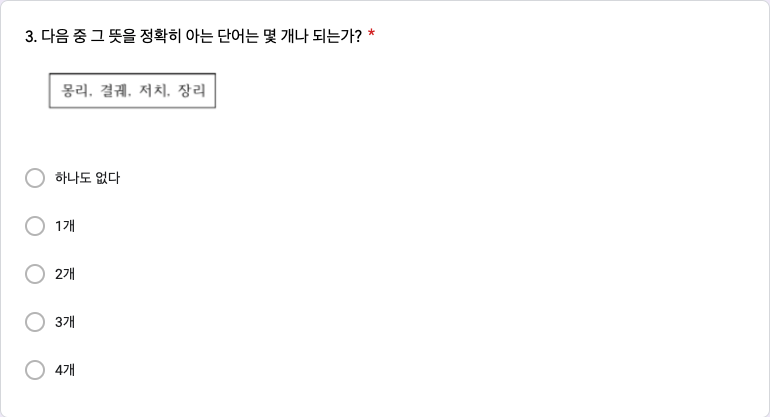
\includegraphics[width=0.75\linewidth]{./pics/Quiz210323_Q3} \end{flushleft}

\subsubsection{몇 개나
아나요?(집계표)}\label{uxba87-uxac1cuxb098-uxc544uxb098uxc694uxc9d1uxacc4uxd45c}

\begin{longtable}[]{@{}
  >{\raggedright\arraybackslash}p{(\columnwidth - 12\tabcolsep) * \real{0.1667}}
  >{\centering\arraybackslash}p{(\columnwidth - 12\tabcolsep) * \real{0.1944}}
  >{\centering\arraybackslash}p{(\columnwidth - 12\tabcolsep) * \real{0.0833}}
  >{\centering\arraybackslash}p{(\columnwidth - 12\tabcolsep) * \real{0.0833}}
  >{\centering\arraybackslash}p{(\columnwidth - 12\tabcolsep) * \real{0.0833}}
  >{\centering\arraybackslash}p{(\columnwidth - 12\tabcolsep) * \real{0.0833}}
  >{\centering\arraybackslash}p{(\columnwidth - 12\tabcolsep) * \real{0.0833}}@{}}
\toprule\noalign{}
\begin{minipage}[b]{\linewidth}\raggedright
~
\end{minipage} & \begin{minipage}[b]{\linewidth}\centering
하나도 없다
\end{minipage} & \begin{minipage}[b]{\linewidth}\centering
1개
\end{minipage} & \begin{minipage}[b]{\linewidth}\centering
2개
\end{minipage} & \begin{minipage}[b]{\linewidth}\centering
3개
\end{minipage} & \begin{minipage}[b]{\linewidth}\centering
4개
\end{minipage} & \begin{minipage}[b]{\linewidth}\centering
계
\end{minipage} \\
\midrule\noalign{}
\endhead
\bottomrule\noalign{}
\endlastfoot
\textbf{Red} & 138 & 72 & 41 & 15 & 11 & 277 \\
\textbf{Black} & 150 & 70 & 40 & 11 & 10 & 281 \\
\textbf{계} & 288 & 142 & 81 & 26 & 21 & 558 \\
\end{longtable}

\begin{longtable}[]{@{}
  >{\raggedleft\arraybackslash}p{(\columnwidth - 4\tabcolsep) * \real{0.2361}}
  >{\raggedleft\arraybackslash}p{(\columnwidth - 4\tabcolsep) * \real{0.0694}}
  >{\raggedleft\arraybackslash}p{(\columnwidth - 4\tabcolsep) * \real{0.1389}}@{}}
\caption{Pearson's Chi-squared test: \texttt{.}}\tabularnewline
\toprule\noalign{}
\begin{minipage}[b]{\linewidth}\raggedleft
Test statistic
\end{minipage} & \begin{minipage}[b]{\linewidth}\raggedleft
df
\end{minipage} & \begin{minipage}[b]{\linewidth}\raggedleft
P value
\end{minipage} \\
\midrule\noalign{}
\endfirsthead
\toprule\noalign{}
\begin{minipage}[b]{\linewidth}\raggedleft
Test statistic
\end{minipage} & \begin{minipage}[b]{\linewidth}\raggedleft
df
\end{minipage} & \begin{minipage}[b]{\linewidth}\raggedleft
P value
\end{minipage} \\
\midrule\noalign{}
\endhead
\bottomrule\noalign{}
\endlastfoot
1.175 & 4 & 0.8822 \\
\end{longtable}

Q3의 집계 결과가 Red, Black 간에 통계적으로 유의한 차이가 있는지
알아보기 위하여 카이제곱 테스트를 수행하였습니다.

그 결과 카이제곱 통계량은 1.175, 자유도는 4, p-value 는 0.8822이므로
Red, Black 간에 통계적으로 유의한 차이를 보이지 않습니다.

실제로 닮은 게 느껴집니까?

\subsubsection{몇 개나
아나요?(\%)}\label{uxba87-uxac1cuxb098-uxc544uxb098uxc694}

\begin{longtable}[]{@{}
  >{\centering\arraybackslash}p{(\columnwidth - 10\tabcolsep) * \real{0.1944}}
  >{\centering\arraybackslash}p{(\columnwidth - 10\tabcolsep) * \real{0.0972}}
  >{\centering\arraybackslash}p{(\columnwidth - 10\tabcolsep) * \real{0.0972}}
  >{\centering\arraybackslash}p{(\columnwidth - 10\tabcolsep) * \real{0.0833}}
  >{\centering\arraybackslash}p{(\columnwidth - 10\tabcolsep) * \real{0.0833}}
  >{\centering\arraybackslash}p{(\columnwidth - 10\tabcolsep) * \real{0.1111}}@{}}
\toprule\noalign{}
\begin{minipage}[b]{\linewidth}\centering
하나도 없다
\end{minipage} & \begin{minipage}[b]{\linewidth}\centering
1개
\end{minipage} & \begin{minipage}[b]{\linewidth}\centering
2개
\end{minipage} & \begin{minipage}[b]{\linewidth}\centering
3개
\end{minipage} & \begin{minipage}[b]{\linewidth}\centering
4개
\end{minipage} & \begin{minipage}[b]{\linewidth}\centering
계
\end{minipage} \\
\midrule\noalign{}
\endhead
\bottomrule\noalign{}
\endlastfoot
51.6 & 25.4 & 14.5 & 4.7 & 3.8 & 100.0 \\
\end{longtable}

물론, 이 문제에는 정답이 없으므로 정답률은 의미가 없습니다.

가장 많은 비율로 응답한 것이 ``하나도 없다''이고 51.6(\%) 입니다.

\subsection{Q4. 해방직후
비문해율}\label{q4.-uxd574uxbc29uxc9c1uxd6c4-uxbe44uxbb38uxd574uxc728}

\begin{flushleft}
\includegraphics[width=0.75\linewidth]{./pics/Quiz210323_Q4} \end{flushleft}

\subsubsection{집계}\label{uxc9d1uxacc4}

\begin{longtable}[]{@{}
  >{\raggedright\arraybackslash}p{(\columnwidth - 12\tabcolsep) * \real{0.1667}}
  >{\raggedleft\arraybackslash}p{(\columnwidth - 12\tabcolsep) * \real{0.0833}}
  >{\raggedleft\arraybackslash}p{(\columnwidth - 12\tabcolsep) * \real{0.0833}}
  >{\raggedleft\arraybackslash}p{(\columnwidth - 12\tabcolsep) * \real{0.0833}}
  >{\raggedleft\arraybackslash}p{(\columnwidth - 12\tabcolsep) * \real{0.0833}}
  >{\raggedleft\arraybackslash}p{(\columnwidth - 12\tabcolsep) * \real{0.0833}}
  >{\centering\arraybackslash}p{(\columnwidth - 12\tabcolsep) * \real{0.0833}}@{}}
\toprule\noalign{}
\begin{minipage}[b]{\linewidth}\raggedright
~
\end{minipage} & \begin{minipage}[b]{\linewidth}\raggedleft
90\%
\end{minipage} & \begin{minipage}[b]{\linewidth}\raggedleft
80\%
\end{minipage} & \begin{minipage}[b]{\linewidth}\raggedleft
50\%
\end{minipage} & \begin{minipage}[b]{\linewidth}\raggedleft
20\%
\end{minipage} & \begin{minipage}[b]{\linewidth}\raggedleft
10\%
\end{minipage} & \begin{minipage}[b]{\linewidth}\centering
계
\end{minipage} \\
\midrule\noalign{}
\endhead
\bottomrule\noalign{}
\endlastfoot
\textbf{Red} & 13 & 198 & 27 & 28 & 11 & 277 \\
\textbf{Black} & 15 & 193 & 35 & 23 & 15 & 281 \\
\textbf{계} & 28 & 391 & 62 & 51 & 26 & 558 \\
\end{longtable}

\begin{longtable}[]{@{}
  >{\raggedleft\arraybackslash}p{(\columnwidth - 4\tabcolsep) * \real{0.2361}}
  >{\raggedleft\arraybackslash}p{(\columnwidth - 4\tabcolsep) * \real{0.0694}}
  >{\raggedleft\arraybackslash}p{(\columnwidth - 4\tabcolsep) * \real{0.1389}}@{}}
\caption{Pearson's Chi-squared test: \texttt{.}}\tabularnewline
\toprule\noalign{}
\begin{minipage}[b]{\linewidth}\raggedleft
Test statistic
\end{minipage} & \begin{minipage}[b]{\linewidth}\raggedleft
df
\end{minipage} & \begin{minipage}[b]{\linewidth}\raggedleft
P value
\end{minipage} \\
\midrule\noalign{}
\endfirsthead
\toprule\noalign{}
\begin{minipage}[b]{\linewidth}\raggedleft
Test statistic
\end{minipage} & \begin{minipage}[b]{\linewidth}\raggedleft
df
\end{minipage} & \begin{minipage}[b]{\linewidth}\raggedleft
P value
\end{minipage} \\
\midrule\noalign{}
\endhead
\bottomrule\noalign{}
\endlastfoot
2.316 & 4 & 0.6778 \\
\end{longtable}

Q4의 집계 결과가 Red, Black 간에 통계적으로 유의한 차이가 있는지
알아보기 위하여 카이제곱 테스트를 수행하였습니다.

그 결과 카이제곱 통계량은 2.316, 자유도는 4, p-value 는 0.6778이므로
Red, Black 간에 통계적으로 유의한 차이를 보이지 않습니다.

실제로 닮은 게 느껴집니까?

\subsubsection{\%}\label{section}

\begin{longtable}[]{@{}
  >{\raggedleft\arraybackslash}p{(\columnwidth - 10\tabcolsep) * \real{0.0833}}
  >{\raggedleft\arraybackslash}p{(\columnwidth - 10\tabcolsep) * \real{0.0972}}
  >{\raggedleft\arraybackslash}p{(\columnwidth - 10\tabcolsep) * \real{0.0972}}
  >{\raggedleft\arraybackslash}p{(\columnwidth - 10\tabcolsep) * \real{0.0833}}
  >{\raggedleft\arraybackslash}p{(\columnwidth - 10\tabcolsep) * \real{0.0833}}
  >{\centering\arraybackslash}p{(\columnwidth - 10\tabcolsep) * \real{0.1111}}@{}}
\toprule\noalign{}
\begin{minipage}[b]{\linewidth}\raggedleft
90\%
\end{minipage} & \begin{minipage}[b]{\linewidth}\raggedleft
80\%
\end{minipage} & \begin{minipage}[b]{\linewidth}\raggedleft
50\%
\end{minipage} & \begin{minipage}[b]{\linewidth}\raggedleft
20\%
\end{minipage} & \begin{minipage}[b]{\linewidth}\raggedleft
10\%
\end{minipage} & \begin{minipage}[b]{\linewidth}\centering
계
\end{minipage} \\
\midrule\noalign{}
\endhead
\bottomrule\noalign{}
\endlastfoot
5.0 & 70.1 & 11.1 & 9.1 & 4.7 & 100.0 \\
\end{longtable}

정답률은 Red, Black 을 합하여 계산하는데, 70.1(\%) 입니다.

\subsection{Q5. 세대간 문해력
격차}\label{q5.-uxc138uxb300uxac04-uxbb38uxd574uxb825-uxaca9uxcc28}

\begin{flushleft}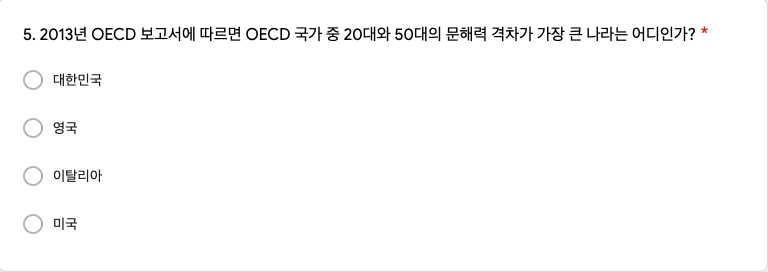
\includegraphics[width=0.75\linewidth]{./pics/Quiz210323_Q5} \end{flushleft}

\subsubsection{집계}\label{uxc9d1uxacc4-1}

\begin{longtable}[]{@{}
  >{\raggedright\arraybackslash}p{(\columnwidth - 10\tabcolsep) * \real{0.1667}}
  >{\centering\arraybackslash}p{(\columnwidth - 10\tabcolsep) * \real{0.1528}}
  >{\centering\arraybackslash}p{(\columnwidth - 10\tabcolsep) * \real{0.0972}}
  >{\centering\arraybackslash}p{(\columnwidth - 10\tabcolsep) * \real{0.1528}}
  >{\centering\arraybackslash}p{(\columnwidth - 10\tabcolsep) * \real{0.0972}}
  >{\centering\arraybackslash}p{(\columnwidth - 10\tabcolsep) * \real{0.0972}}@{}}
\toprule\noalign{}
\begin{minipage}[b]{\linewidth}\raggedright
~
\end{minipage} & \begin{minipage}[b]{\linewidth}\centering
대한민국
\end{minipage} & \begin{minipage}[b]{\linewidth}\centering
영국
\end{minipage} & \begin{minipage}[b]{\linewidth}\centering
이탈리아
\end{minipage} & \begin{minipage}[b]{\linewidth}\centering
미국
\end{minipage} & \begin{minipage}[b]{\linewidth}\centering
계
\end{minipage} \\
\midrule\noalign{}
\endhead
\bottomrule\noalign{}
\endlastfoot
\textbf{Red} & 212 & 18 & 18 & 29 & 277 \\
\textbf{Black} & 219 & 14 & 15 & 33 & 281 \\
\textbf{계} & 431 & 32 & 33 & 62 & 558 \\
\end{longtable}

\begin{longtable}[]{@{}
  >{\raggedleft\arraybackslash}p{(\columnwidth - 4\tabcolsep) * \real{0.2361}}
  >{\raggedleft\arraybackslash}p{(\columnwidth - 4\tabcolsep) * \real{0.0694}}
  >{\raggedleft\arraybackslash}p{(\columnwidth - 4\tabcolsep) * \real{0.1389}}@{}}
\caption{Pearson's Chi-squared test: \texttt{.}}\tabularnewline
\toprule\noalign{}
\begin{minipage}[b]{\linewidth}\raggedleft
Test statistic
\end{minipage} & \begin{minipage}[b]{\linewidth}\raggedleft
df
\end{minipage} & \begin{minipage}[b]{\linewidth}\raggedleft
P value
\end{minipage} \\
\midrule\noalign{}
\endfirsthead
\toprule\noalign{}
\begin{minipage}[b]{\linewidth}\raggedleft
Test statistic
\end{minipage} & \begin{minipage}[b]{\linewidth}\raggedleft
df
\end{minipage} & \begin{minipage}[b]{\linewidth}\raggedleft
P value
\end{minipage} \\
\midrule\noalign{}
\endhead
\bottomrule\noalign{}
\endlastfoot
1.116 & 3 & 0.7732 \\
\end{longtable}

Q5의 집계 결과가 Red, Black 간에 통계적으로 유의한 차이가 있는지
알아보기 위하여 카이제곱 테스트를 수행하였습니다.

그 결과 카이제곱 통계량은 1.116, 자유도는 3, p-value 는 0.7732이므로
Red, Black 간에 통계적으로 유의한 차이를 보이지 않습니다.

실제로 닮은 게 느껴집니까?

\subsubsection{\%}\label{section-1}

\begin{longtable}[]{@{}
  >{\centering\arraybackslash}p{(\columnwidth - 8\tabcolsep) * \real{0.1528}}
  >{\centering\arraybackslash}p{(\columnwidth - 8\tabcolsep) * \real{0.0972}}
  >{\centering\arraybackslash}p{(\columnwidth - 8\tabcolsep) * \real{0.1528}}
  >{\centering\arraybackslash}p{(\columnwidth - 8\tabcolsep) * \real{0.0972}}
  >{\centering\arraybackslash}p{(\columnwidth - 8\tabcolsep) * \real{0.1111}}@{}}
\toprule\noalign{}
\begin{minipage}[b]{\linewidth}\centering
대한민국
\end{minipage} & \begin{minipage}[b]{\linewidth}\centering
영국
\end{minipage} & \begin{minipage}[b]{\linewidth}\centering
이탈리아
\end{minipage} & \begin{minipage}[b]{\linewidth}\centering
미국
\end{minipage} & \begin{minipage}[b]{\linewidth}\centering
계
\end{minipage} \\
\midrule\noalign{}
\endhead
\bottomrule\noalign{}
\endlastfoot
77.2 & 5.7 & 5.9 & 11.1 & 100.0 \\
\end{longtable}

정답률은 Red, Black 을 합하여 계산하는데, 77.2(\%) 입니다.

\subsection{Q6. 문해력 격차의
파급효과}\label{q6.-uxbb38uxd574uxb825-uxaca9uxcc28uxc758-uxd30cuxae09uxd6a8uxacfc}

\begin{flushleft}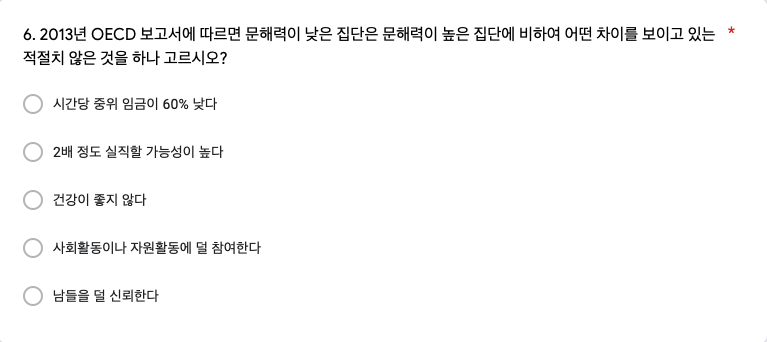
\includegraphics[width=0.75\linewidth]{./pics/Quiz210323_Q6} \end{flushleft}

\subsubsection{집계}\label{uxc9d1uxacc4-2}

\begin{longtable}[]{@{}
  >{\raggedright\arraybackslash}p{(\columnwidth - 12\tabcolsep) * \real{0.1463}}
  >{\centering\arraybackslash}p{(\columnwidth - 12\tabcolsep) * \real{0.1951}}
  >{\centering\arraybackslash}p{(\columnwidth - 12\tabcolsep) * \real{0.1707}}
  >{\centering\arraybackslash}p{(\columnwidth - 12\tabcolsep) * \real{0.1463}}
  >{\centering\arraybackslash}p{(\columnwidth - 12\tabcolsep) * \real{0.1463}}
  >{\centering\arraybackslash}p{(\columnwidth - 12\tabcolsep) * \real{0.1220}}
  >{\centering\arraybackslash}p{(\columnwidth - 12\tabcolsep) * \real{0.0732}}@{}}
\toprule\noalign{}
\begin{minipage}[b]{\linewidth}\raggedright
~
\end{minipage} & \begin{minipage}[b]{\linewidth}\centering
60\% 낮은 임금
\end{minipage} & \begin{minipage}[b]{\linewidth}\centering
실직 가능성
\end{minipage} & \begin{minipage}[b]{\linewidth}\centering
나쁜 건강
\end{minipage} & \begin{minipage}[b]{\linewidth}\centering
활동 불참
\end{minipage} & \begin{minipage}[b]{\linewidth}\centering
덜 신뢰
\end{minipage} & \begin{minipage}[b]{\linewidth}\centering
계
\end{minipage} \\
\midrule\noalign{}
\endhead
\bottomrule\noalign{}
\endlastfoot
\textbf{Red} & 153 & 24 & 40 & 23 & 37 & 277 \\
\textbf{Black} & 152 & 20 & 39 & 20 & 50 & 281 \\
\textbf{계} & 305 & 44 & 79 & 43 & 87 & 558 \\
\end{longtable}

\begin{longtable}[]{@{}
  >{\raggedleft\arraybackslash}p{(\columnwidth - 4\tabcolsep) * \real{0.2361}}
  >{\raggedleft\arraybackslash}p{(\columnwidth - 4\tabcolsep) * \real{0.0694}}
  >{\raggedleft\arraybackslash}p{(\columnwidth - 4\tabcolsep) * \real{0.1389}}@{}}
\caption{Pearson's Chi-squared test: \texttt{.}}\tabularnewline
\toprule\noalign{}
\begin{minipage}[b]{\linewidth}\raggedleft
Test statistic
\end{minipage} & \begin{minipage}[b]{\linewidth}\raggedleft
df
\end{minipage} & \begin{minipage}[b]{\linewidth}\raggedleft
P value
\end{minipage} \\
\midrule\noalign{}
\endfirsthead
\toprule\noalign{}
\begin{minipage}[b]{\linewidth}\raggedleft
Test statistic
\end{minipage} & \begin{minipage}[b]{\linewidth}\raggedleft
df
\end{minipage} & \begin{minipage}[b]{\linewidth}\raggedleft
P value
\end{minipage} \\
\midrule\noalign{}
\endhead
\bottomrule\noalign{}
\endlastfoot
2.503 & 4 & 0.6441 \\
\end{longtable}

Q6의 집계 결과가 Red, Black 간에 통계적으로 유의한 차이가 있는지
알아보기 위하여 카이제곱 테스트를 수행하였습니다.

그 결과 카이제곱 통계량은 2.503, 자유도는 4, p-value 는 0.6441이므로
Red, Black 간에 통계적으로 유의한 차이를 보이지 않습니다.

실제로 닮은 게 느껴집니까?

\subsubsection{\%}\label{section-2}

\begin{longtable}[]{@{}
  >{\centering\arraybackslash}p{(\columnwidth - 10\tabcolsep) * \real{0.2162}}
  >{\centering\arraybackslash}p{(\columnwidth - 10\tabcolsep) * \real{0.1892}}
  >{\centering\arraybackslash}p{(\columnwidth - 10\tabcolsep) * \real{0.1622}}
  >{\centering\arraybackslash}p{(\columnwidth - 10\tabcolsep) * \real{0.1622}}
  >{\centering\arraybackslash}p{(\columnwidth - 10\tabcolsep) * \real{0.1351}}
  >{\centering\arraybackslash}p{(\columnwidth - 10\tabcolsep) * \real{0.1351}}@{}}
\toprule\noalign{}
\begin{minipage}[b]{\linewidth}\centering
60\% 낮은 임금
\end{minipage} & \begin{minipage}[b]{\linewidth}\centering
실직 가능성
\end{minipage} & \begin{minipage}[b]{\linewidth}\centering
나쁜 건강
\end{minipage} & \begin{minipage}[b]{\linewidth}\centering
활동 불참
\end{minipage} & \begin{minipage}[b]{\linewidth}\centering
덜 신뢰
\end{minipage} & \begin{minipage}[b]{\linewidth}\centering
계
\end{minipage} \\
\midrule\noalign{}
\endhead
\bottomrule\noalign{}
\endlastfoot
54.7 & 7.9 & 14.2 & 7.7 & 15.6 & 100.0 \\
\end{longtable}

정답률은 Red, Black 을 합하여 계산하는데, 54.7(\%) 입니다.

\subsection{Q7. 프레임을 설정하는 단어의
힘}\label{q7.-uxd504uxb808uxc784uxc744-uxc124uxc815uxd558uxb294-uxb2e8uxc5b4uxc758-uxd798}

컵 가득 음료수를 채웠는데 미끄러지면서 반을 쏟았습니다.

이 상황에서 어떤 사람은 ``그래도 반이 남았네''라고 긍정적 반응을 하고 또
다른 사람은 ``어쩌나 반 밖에 안 남았네''라고 부정적 반응을 보일 수
있습니다.

만약, 반응을 보이기 전에 Red 에는 긍정적 단어들을 읽게 하고, Black 에는
부정적 단어들을 읽게 한 후 반응을 물어보면 어떻게 될까요?

Red, Black 의 성격상 단어를 보기 전에는 긍정적 반응의 비율과 부정적
반응의 비율이 닮을 것으로 기대됩니다.

그러나 단어를 보고 나서는 반응이 극명하게 나뉘는 것을 관찰하게 됩니다.

통계적으로 매우, 매우, \ldots{} 유의한 차이를 보여 줍니다.

이것도 일종의 프레이밍이 인식에 미치는 영향이라고 할 수 있겠습니다.

힘든 상황이라도 긍정적인 생각을 가져야겠죠?

\begin{flushleft}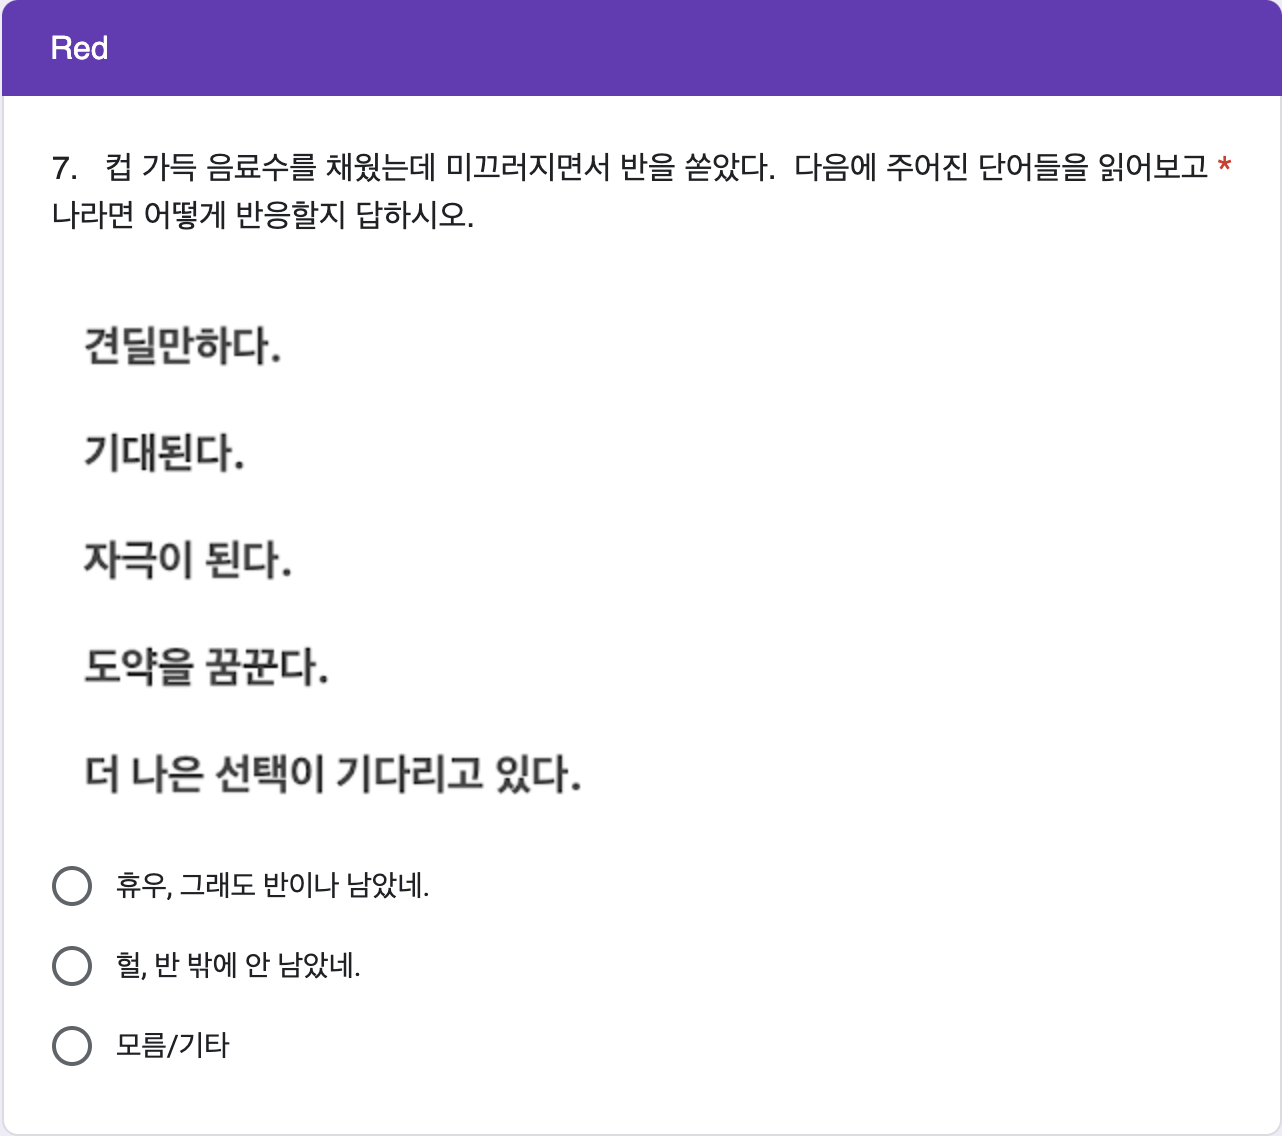
\includegraphics[width=0.67\linewidth]{./pics/Quiz240329_Q7_Red} \end{flushleft}

\begin{flushleft}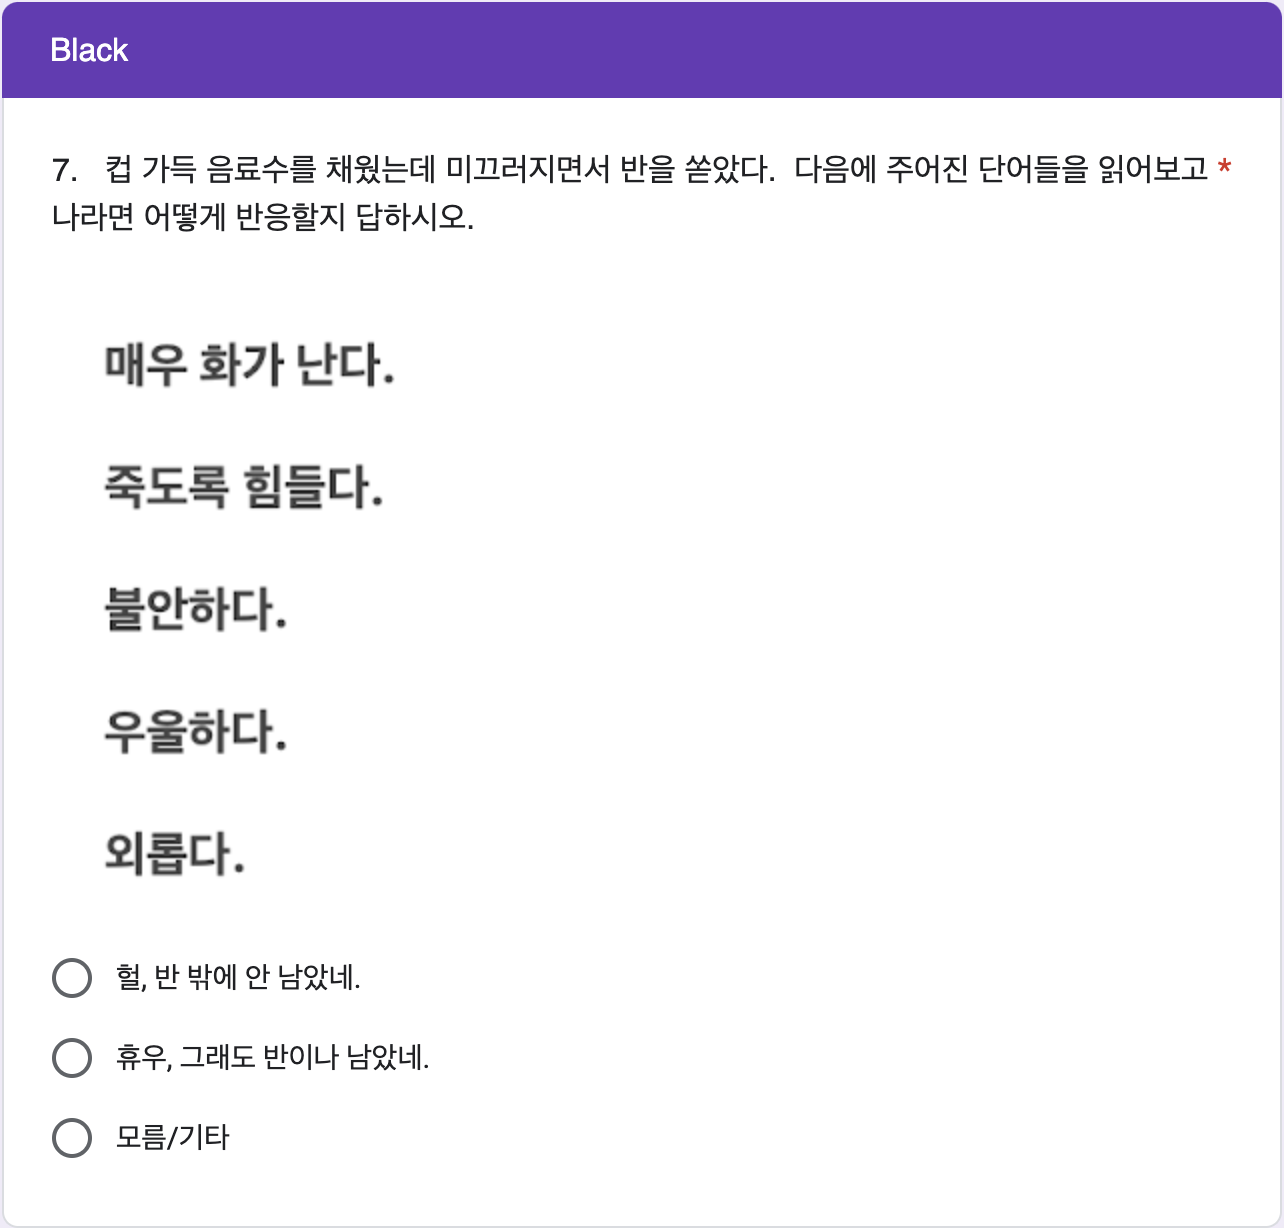
\includegraphics[width=0.67\linewidth]{./pics/Quiz240329_Q7_Black} \end{flushleft}

\subsubsection{집계}\label{uxc9d1uxacc4-3}

\begin{longtable}[]{@{}
  >{\raggedright\arraybackslash}p{(\columnwidth - 8\tabcolsep) * \real{0.3472}}
  >{\centering\arraybackslash}p{(\columnwidth - 8\tabcolsep) * \real{0.1250}}
  >{\centering\arraybackslash}p{(\columnwidth - 8\tabcolsep) * \real{0.1250}}
  >{\centering\arraybackslash}p{(\columnwidth - 8\tabcolsep) * \real{0.1667}}
  >{\centering\arraybackslash}p{(\columnwidth - 8\tabcolsep) * \real{0.0833}}@{}}
\toprule\noalign{}
\begin{minipage}[b]{\linewidth}\raggedright
~
\end{minipage} & \begin{minipage}[b]{\linewidth}\centering
반이나
\end{minipage} & \begin{minipage}[b]{\linewidth}\centering
반밖에
\end{minipage} & \begin{minipage}[b]{\linewidth}\centering
모름/기타
\end{minipage} & \begin{minipage}[b]{\linewidth}\centering
계
\end{minipage} \\
\midrule\noalign{}
\endhead
\bottomrule\noalign{}
\endlastfoot
\textbf{Red(긍정적 단어)} & 213 & 49 & 15 & 277 \\
\textbf{Black(부정적 단어)} & 83 & 183 & 15 & 281 \\
\textbf{계} & 296 & 232 & 30 & 558 \\
\end{longtable}

\begin{longtable}[]{@{}
  >{\raggedleft\arraybackslash}p{(\columnwidth - 4\tabcolsep) * \real{0.2361}}
  >{\raggedleft\arraybackslash}p{(\columnwidth - 4\tabcolsep) * \real{0.0694}}
  >{\raggedleft\arraybackslash}p{(\columnwidth - 4\tabcolsep) * \real{0.2500}}@{}}
\caption{Pearson's Chi-squared test: \texttt{.}}\tabularnewline
\toprule\noalign{}
\begin{minipage}[b]{\linewidth}\raggedleft
Test statistic
\end{minipage} & \begin{minipage}[b]{\linewidth}\raggedleft
df
\end{minipage} & \begin{minipage}[b]{\linewidth}\raggedleft
P value
\end{minipage} \\
\midrule\noalign{}
\endfirsthead
\toprule\noalign{}
\begin{minipage}[b]{\linewidth}\raggedleft
Test statistic
\end{minipage} & \begin{minipage}[b]{\linewidth}\raggedleft
df
\end{minipage} & \begin{minipage}[b]{\linewidth}\raggedleft
P value
\end{minipage} \\
\midrule\noalign{}
\endhead
\bottomrule\noalign{}
\endlastfoot
134.5 & 2 & 6.315e-30 * * * \\
\end{longtable}

Q7의 Red는 음료수를 쏟은 상황에서 ``견딜만 하다'' 등의 긍정적인 단어들을
본 사람들인 데 277명이 응답한 가운데 213명이 ``반이나'' 남아 있다는
반응을 보이고, 49명이 ``반 밖에'' 안 남았다는 반응을 보입니다.

Black은 같은 상황에서 ``매우 화가 난다'' 등의 부정적인 단어들을 본
사람들인 데 281명이 응답한 가운데 83명이 ``반이나'' 남아 있다는 반응을
보이고, 183명이 ``반 밖에'' 안 남았다는 반응을 보입니다.

그리고 ``모름/기타''에 답한 인원은 Red에 15명, Black 에 15명이었습니다.

랜덤화 효과일까요?

``모름/기타''의 응답이 유난히 닮은 게 이런 해석을 불러 일으킵니다.

카이제곱 테스트는 이와 같은 상황에서 단어들을 이용하여 긍정적인 프레임을
구성한 경우와 부정적인 프레임을 구성한 경우에 그 차이가 통계적으로 매우,
매우, \ldots{} 유의하다는 것을 보여 줍니다.

카이제곱 통계량은 134.469, 자유도는 2, p-value 는 6.3e-30 긍정적인
단어나 부정적인 단어를 단지 읽는 것만으로도 프레임이 설정되어 반응이
다르게 나온다는 것을 보여줍니다.

여기서 긍정이나 부정 프레이밍이 응답에 영향을 끼치지 않는다고 가정해
봅시다.

그렇다면 Red, Black 의 응답은 Q1 \textasciitilde{} Q6에서와 같이 랜덤화
효과에 의하여 통계적으로 유의한 차이를 보이지 않을 것입니다.

그런데 실제로 관찰된 카이제곱 통계값은 통계적으로 매우 유의한 차이를
보여 줍니다.

따라서 긍정이나 부정 프레이밍이 영향을 끼치지 않는다는 가정이
잘못되었다는 것을 논리적으로 입증할 수 있습니다.

이러한 논증 방식을 귀류법이라 합니다.

\subsubsection{\% 비교.}\label{uxbe44uxad50.}

\begin{longtable}[]{@{}
  >{\raggedright\arraybackslash}p{(\columnwidth - 8\tabcolsep) * \real{0.3472}}
  >{\centering\arraybackslash}p{(\columnwidth - 8\tabcolsep) * \real{0.1250}}
  >{\centering\arraybackslash}p{(\columnwidth - 8\tabcolsep) * \real{0.1250}}
  >{\centering\arraybackslash}p{(\columnwidth - 8\tabcolsep) * \real{0.1667}}
  >{\centering\arraybackslash}p{(\columnwidth - 8\tabcolsep) * \real{0.1111}}@{}}
\toprule\noalign{}
\begin{minipage}[b]{\linewidth}\raggedright
~
\end{minipage} & \begin{minipage}[b]{\linewidth}\centering
반이나
\end{minipage} & \begin{minipage}[b]{\linewidth}\centering
반밖에
\end{minipage} & \begin{minipage}[b]{\linewidth}\centering
모름/기타
\end{minipage} & \begin{minipage}[b]{\linewidth}\centering
계
\end{minipage} \\
\midrule\noalign{}
\endhead
\bottomrule\noalign{}
\endlastfoot
\textbf{Red(긍정적 단어)} & 76.9 & 17.7 & 5.4 & 100.0 \\
\textbf{Black(부정적 단어)} & 29.5 & 65.1 & 5.3 & 100.0 \\
\end{longtable}

긍정적인 단어들을 읽어 본 Red에서 ``반이나'' 남았다고 응답하는사람들의
백분율, 76.9(\%)은 ``반 밖에'' 안 남았다고 응답하는 사람들의 백분율,
17.7(\%) 보다 월등히 높습니다.

반면 부정적인 단어들을 읽어 본 Black에서 ``반이나'' 남았다고
응답하는사람들의 백분율, 29.5(\%)은 ``반 밖에'' 안 남았다고 응답하는
사람들의 백분율, 65.1(\%) 보다 훨씬 적습니다.

긍정적인 단어를 읽느냐, 부정적인 단어를 읽느냐에 따라 형성된 프레임의
영향이 막대하다는 것을 잘 알 수 있습니다.

Red 와 Black 이 워낙 차이가 나지만 전체적으로 어느 정도가 ``반이나''
남았다, 혹은 ``반 밖에'' 안 남았다고 응답하였는지 합쳐 보겠습니다.

\subsubsection{\% 합산}\label{uxd569uxc0b0}

\begin{longtable}[]{@{}
  >{\centering\arraybackslash}p{(\columnwidth - 6\tabcolsep) * \real{0.1250}}
  >{\centering\arraybackslash}p{(\columnwidth - 6\tabcolsep) * \real{0.1250}}
  >{\centering\arraybackslash}p{(\columnwidth - 6\tabcolsep) * \real{0.1667}}
  >{\centering\arraybackslash}p{(\columnwidth - 6\tabcolsep) * \real{0.1111}}@{}}
\toprule\noalign{}
\begin{minipage}[b]{\linewidth}\centering
반이나
\end{minipage} & \begin{minipage}[b]{\linewidth}\centering
반밖에
\end{minipage} & \begin{minipage}[b]{\linewidth}\centering
모름/기타
\end{minipage} & \begin{minipage}[b]{\linewidth}\centering
계
\end{minipage} \\
\midrule\noalign{}
\endhead
\bottomrule\noalign{}
\endlastfoot
53.0 & 41.6 & 5.4 & 100.0 \\
\end{longtable}

``반이나'' 남아 있다고 응답한 백분율은 Red, Black 합쳐서 53.0(\%)(으)로
'반 밖에 '' 안 남아 있다고 응답한 백분율, 41.6(\%) 보다 상당히 많습니다.

\subsubsection{Mosaic Plot}\label{mosaic-plot}


\includegraphics{quiz250331_Report_v4_files/figure-latex/mosaic plot-1.pdf}

Mosaic Plot 은 이 집계결과를 시각적으로 잘 보여줍니다. 긍정적 단어를 본
Red 에서 ``반이나'' 남아 있다고 응답한 백분율이 월등히 높고, 부정적
단어를 본 Black 에서 ``반 밖에'' 안 남았다고 응답한 백분율이 월등히 높은
것을 시각적으로 알 수 있습니다.

덤으로 ``모름/기타''의 백분율은 Red, Black 간에 매우 닮았다는 점도
시각적으로 쉽게 파악할 수 있습니다.

\subsection{마감 시간으로부터 제출 시간의
분포}\label{uxb9c8uxac10-uxc2dcuxac04uxc73cuxb85cuxbd80uxd130-uxc81cuxcd9c-uxc2dcuxac04uxc758-uxbd84uxd3ec}

\subsubsection{분포표}\label{uxbd84uxd3ecuxd45c}

\begin{longtable}[]{@{}
  >{\raggedright\arraybackslash}p{(\columnwidth - 30\tabcolsep) * \real{0.0863}}
  >{\raggedleft\arraybackslash}p{(\columnwidth - 30\tabcolsep) * \real{0.0576}}
  >{\raggedleft\arraybackslash}p{(\columnwidth - 30\tabcolsep) * \real{0.0576}}
  >{\raggedleft\arraybackslash}p{(\columnwidth - 30\tabcolsep) * \real{0.0576}}
  >{\raggedleft\arraybackslash}p{(\columnwidth - 30\tabcolsep) * \real{0.0576}}
  >{\raggedleft\arraybackslash}p{(\columnwidth - 30\tabcolsep) * \real{0.0576}}
  >{\raggedleft\arraybackslash}p{(\columnwidth - 30\tabcolsep) * \real{0.0576}}
  >{\raggedleft\arraybackslash}p{(\columnwidth - 30\tabcolsep) * \real{0.0576}}
  >{\raggedleft\arraybackslash}p{(\columnwidth - 30\tabcolsep) * \real{0.0576}}
  >{\raggedleft\arraybackslash}p{(\columnwidth - 30\tabcolsep) * \real{0.0576}}
  >{\raggedleft\arraybackslash}p{(\columnwidth - 30\tabcolsep) * \real{0.0647}}
  >{\raggedleft\arraybackslash}p{(\columnwidth - 30\tabcolsep) * \real{0.0719}}
  >{\raggedleft\arraybackslash}p{(\columnwidth - 30\tabcolsep) * \real{0.0719}}
  >{\raggedleft\arraybackslash}p{(\columnwidth - 30\tabcolsep) * \real{0.0719}}
  >{\raggedleft\arraybackslash}p{(\columnwidth - 30\tabcolsep) * \real{0.0719}}
  >{\centering\arraybackslash}p{(\columnwidth - 30\tabcolsep) * \real{0.0432}}@{}}
\caption{일 단위}\tabularnewline
\toprule\noalign{}
\begin{minipage}[b]{\linewidth}\raggedright
~
\end{minipage} & \begin{minipage}[b]{\linewidth}\raggedleft
{[}0,1{]}
\end{minipage} & \begin{minipage}[b]{\linewidth}\raggedleft
(1,2{]}
\end{minipage} & \begin{minipage}[b]{\linewidth}\raggedleft
(2,3{]}
\end{minipage} & \begin{minipage}[b]{\linewidth}\raggedleft
(3,4{]}
\end{minipage} & \begin{minipage}[b]{\linewidth}\raggedleft
(4,5{]}
\end{minipage} & \begin{minipage}[b]{\linewidth}\raggedleft
(5,6{]}
\end{minipage} & \begin{minipage}[b]{\linewidth}\raggedleft
(6,7{]}
\end{minipage} & \begin{minipage}[b]{\linewidth}\raggedleft
(7,8{]}
\end{minipage} & \begin{minipage}[b]{\linewidth}\raggedleft
(8,9{]}
\end{minipage} & \begin{minipage}[b]{\linewidth}\raggedleft
(9,10{]}
\end{minipage} & \begin{minipage}[b]{\linewidth}\raggedleft
(10,11{]}
\end{minipage} & \begin{minipage}[b]{\linewidth}\raggedleft
(11,12{]}
\end{minipage} & \begin{minipage}[b]{\linewidth}\raggedleft
(12,13{]}
\end{minipage} & \begin{minipage}[b]{\linewidth}\raggedleft
(13,14{]}
\end{minipage} & \begin{minipage}[b]{\linewidth}\centering
계
\end{minipage} \\
\midrule\noalign{}
\endfirsthead
\toprule\noalign{}
\begin{minipage}[b]{\linewidth}\raggedright
~
\end{minipage} & \begin{minipage}[b]{\linewidth}\raggedleft
{[}0,1{]}
\end{minipage} & \begin{minipage}[b]{\linewidth}\raggedleft
(1,2{]}
\end{minipage} & \begin{minipage}[b]{\linewidth}\raggedleft
(2,3{]}
\end{minipage} & \begin{minipage}[b]{\linewidth}\raggedleft
(3,4{]}
\end{minipage} & \begin{minipage}[b]{\linewidth}\raggedleft
(4,5{]}
\end{minipage} & \begin{minipage}[b]{\linewidth}\raggedleft
(5,6{]}
\end{minipage} & \begin{minipage}[b]{\linewidth}\raggedleft
(6,7{]}
\end{minipage} & \begin{minipage}[b]{\linewidth}\raggedleft
(7,8{]}
\end{minipage} & \begin{minipage}[b]{\linewidth}\raggedleft
(8,9{]}
\end{minipage} & \begin{minipage}[b]{\linewidth}\raggedleft
(9,10{]}
\end{minipage} & \begin{minipage}[b]{\linewidth}\raggedleft
(10,11{]}
\end{minipage} & \begin{minipage}[b]{\linewidth}\raggedleft
(11,12{]}
\end{minipage} & \begin{minipage}[b]{\linewidth}\raggedleft
(12,13{]}
\end{minipage} & \begin{minipage}[b]{\linewidth}\raggedleft
(13,14{]}
\end{minipage} & \begin{minipage}[b]{\linewidth}\centering
계
\end{minipage} \\
\midrule\noalign{}
\endhead
\bottomrule\noalign{}
\endlastfoot
\textbf{Red} & 81 & 14 & 8 & 13 & 11 & 5 & 4 & 38 & 22 & 13 & 14 & 19 &
12 & 23 & 277 \\
\textbf{Black} & 78 & 14 & 12 & 6 & 8 & 3 & 6 & 41 & 29 & 15 & 17 & 15 &
20 & 17 & 281 \\
\textbf{계} & 159 & 28 & 20 & 19 & 19 & 8 & 10 & 79 & 51 & 28 & 31 & 34
& 32 & 40 & 558 \\
\end{longtable}

분포표로부터 두 가지 문제를 살펴보겠습니다.

첫째, 날마다 고르게 제출하는가?

둘째, Red, Black 간에 통계적으로 유의한 차이가 있는가?

각 문제를 살펴보기 위해서는 분포표의 일부분을 대상으로 카이제곱 테스트를
수행합니다.

\subsubsection{날마다 고르게
제출하는가?}\label{uxb0a0uxb9c8uxb2e4-uxace0uxb974uxac8c-uxc81cuxcd9cuxd558uxb294uxac00}

\begin{longtable}[]{@{}
  >{\raggedleft\arraybackslash}p{(\columnwidth - 26\tabcolsep) * \real{0.0661}}
  >{\raggedleft\arraybackslash}p{(\columnwidth - 26\tabcolsep) * \real{0.0661}}
  >{\raggedleft\arraybackslash}p{(\columnwidth - 26\tabcolsep) * \real{0.0661}}
  >{\raggedleft\arraybackslash}p{(\columnwidth - 26\tabcolsep) * \real{0.0661}}
  >{\raggedleft\arraybackslash}p{(\columnwidth - 26\tabcolsep) * \real{0.0661}}
  >{\raggedleft\arraybackslash}p{(\columnwidth - 26\tabcolsep) * \real{0.0661}}
  >{\raggedleft\arraybackslash}p{(\columnwidth - 26\tabcolsep) * \real{0.0661}}
  >{\raggedleft\arraybackslash}p{(\columnwidth - 26\tabcolsep) * \real{0.0661}}
  >{\raggedleft\arraybackslash}p{(\columnwidth - 26\tabcolsep) * \real{0.0661}}
  >{\raggedleft\arraybackslash}p{(\columnwidth - 26\tabcolsep) * \real{0.0744}}
  >{\raggedleft\arraybackslash}p{(\columnwidth - 26\tabcolsep) * \real{0.0826}}
  >{\raggedleft\arraybackslash}p{(\columnwidth - 26\tabcolsep) * \real{0.0826}}
  >{\raggedleft\arraybackslash}p{(\columnwidth - 26\tabcolsep) * \real{0.0826}}
  >{\raggedleft\arraybackslash}p{(\columnwidth - 26\tabcolsep) * \real{0.0826}}@{}}
\toprule\noalign{}
\begin{minipage}[b]{\linewidth}\raggedleft
{[}0,1{]}
\end{minipage} & \begin{minipage}[b]{\linewidth}\raggedleft
(1,2{]}
\end{minipage} & \begin{minipage}[b]{\linewidth}\raggedleft
(2,3{]}
\end{minipage} & \begin{minipage}[b]{\linewidth}\raggedleft
(3,4{]}
\end{minipage} & \begin{minipage}[b]{\linewidth}\raggedleft
(4,5{]}
\end{minipage} & \begin{minipage}[b]{\linewidth}\raggedleft
(5,6{]}
\end{minipage} & \begin{minipage}[b]{\linewidth}\raggedleft
(6,7{]}
\end{minipage} & \begin{minipage}[b]{\linewidth}\raggedleft
(7,8{]}
\end{minipage} & \begin{minipage}[b]{\linewidth}\raggedleft
(8,9{]}
\end{minipage} & \begin{minipage}[b]{\linewidth}\raggedleft
(9,10{]}
\end{minipage} & \begin{minipage}[b]{\linewidth}\raggedleft
(10,11{]}
\end{minipage} & \begin{minipage}[b]{\linewidth}\raggedleft
(11,12{]}
\end{minipage} & \begin{minipage}[b]{\linewidth}\raggedleft
(12,13{]}
\end{minipage} & \begin{minipage}[b]{\linewidth}\raggedleft
(13,14{]}
\end{minipage} \\
\midrule\noalign{}
\endhead
\bottomrule\noalign{}
\endlastfoot
159 & 28 & 20 & 19 & 19 & 8 & 10 & 79 & 51 & 28 & 31 & 34 & 32 & 40 \\
\end{longtable}

\begin{longtable}[]{@{}
  >{\raggedleft\arraybackslash}p{(\columnwidth - 4\tabcolsep) * \real{0.2361}}
  >{\raggedleft\arraybackslash}p{(\columnwidth - 4\tabcolsep) * \real{0.0694}}
  >{\raggedleft\arraybackslash}p{(\columnwidth - 4\tabcolsep) * \real{0.2500}}@{}}
\caption{Chi-squared test for given probabilities:
\texttt{.}}\tabularnewline
\toprule\noalign{}
\begin{minipage}[b]{\linewidth}\raggedleft
Test statistic
\end{minipage} & \begin{minipage}[b]{\linewidth}\raggedleft
df
\end{minipage} & \begin{minipage}[b]{\linewidth}\raggedleft
P value
\end{minipage} \\
\midrule\noalign{}
\endfirsthead
\toprule\noalign{}
\begin{minipage}[b]{\linewidth}\raggedleft
Test statistic
\end{minipage} & \begin{minipage}[b]{\linewidth}\raggedleft
df
\end{minipage} & \begin{minipage}[b]{\linewidth}\raggedleft
P value
\end{minipage} \\
\midrule\noalign{}
\endhead
\bottomrule\noalign{}
\endlastfoot
488.7 & 13 & 3.693e-96 * * * \\
\end{longtable}

날마다 고르게 제출하는지 알아 보았습니다.

분포표의 ``계''행에서 '계'열을 제외하고 카이제곱테스트를 수행합니다.
분포표 만으로도 쉽게 파악할 수 있지만 카이제곱테스트가 명확히 해 줍니다.

카이제곱 통계량은 488.69, 자유도는 13.00, p-value 는 3.7e-96 이므로 결코
고르게 제출한다고 말할 수 없겠습니다.

막대그래프로 살펴 보겠습니다.

\subsubsection{막대그래프}\label{uxb9c9uxb300uxadf8uxb798uxd504}

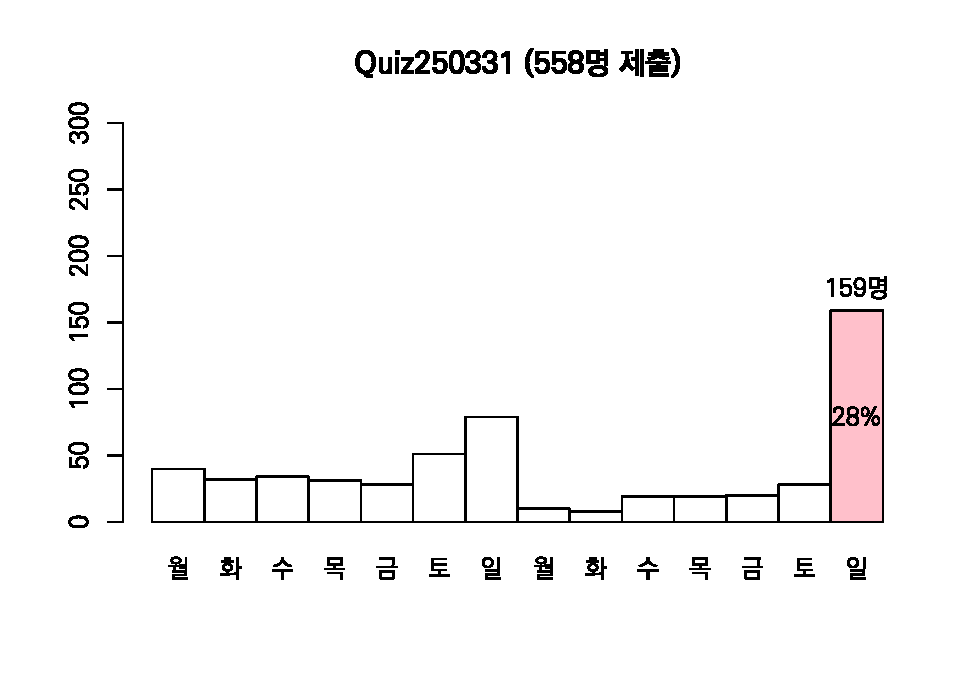
\includegraphics{quiz250331_Report_v4_files/figure-latex/unnamed-chunk-20-1.pdf}

막대그래프는 총 제출인원 558(명) 중에 159(명), 28(\%)가 마감일에 몰리는
것을 명확히 보여주고 있습니다.

\subsubsection{Red, Black 간에
닮았는가?}\label{red-black-uxac04uxc5d0-uxb2eeuxc558uxb294uxac00}

\begin{longtable}[]{@{}
  >{\raggedright\arraybackslash}p{(\columnwidth - 28\tabcolsep) * \real{0.0902}}
  >{\raggedleft\arraybackslash}p{(\columnwidth - 28\tabcolsep) * \real{0.0602}}
  >{\raggedleft\arraybackslash}p{(\columnwidth - 28\tabcolsep) * \real{0.0602}}
  >{\raggedleft\arraybackslash}p{(\columnwidth - 28\tabcolsep) * \real{0.0602}}
  >{\raggedleft\arraybackslash}p{(\columnwidth - 28\tabcolsep) * \real{0.0602}}
  >{\raggedleft\arraybackslash}p{(\columnwidth - 28\tabcolsep) * \real{0.0602}}
  >{\raggedleft\arraybackslash}p{(\columnwidth - 28\tabcolsep) * \real{0.0602}}
  >{\raggedleft\arraybackslash}p{(\columnwidth - 28\tabcolsep) * \real{0.0602}}
  >{\raggedleft\arraybackslash}p{(\columnwidth - 28\tabcolsep) * \real{0.0602}}
  >{\raggedleft\arraybackslash}p{(\columnwidth - 28\tabcolsep) * \real{0.0602}}
  >{\raggedleft\arraybackslash}p{(\columnwidth - 28\tabcolsep) * \real{0.0677}}
  >{\raggedleft\arraybackslash}p{(\columnwidth - 28\tabcolsep) * \real{0.0752}}
  >{\raggedleft\arraybackslash}p{(\columnwidth - 28\tabcolsep) * \real{0.0752}}
  >{\raggedleft\arraybackslash}p{(\columnwidth - 28\tabcolsep) * \real{0.0752}}
  >{\raggedleft\arraybackslash}p{(\columnwidth - 28\tabcolsep) * \real{0.0752}}@{}}
\toprule\noalign{}
\begin{minipage}[b]{\linewidth}\raggedright
~
\end{minipage} & \begin{minipage}[b]{\linewidth}\raggedleft
{[}0,1{]}
\end{minipage} & \begin{minipage}[b]{\linewidth}\raggedleft
(1,2{]}
\end{minipage} & \begin{minipage}[b]{\linewidth}\raggedleft
(2,3{]}
\end{minipage} & \begin{minipage}[b]{\linewidth}\raggedleft
(3,4{]}
\end{minipage} & \begin{minipage}[b]{\linewidth}\raggedleft
(4,5{]}
\end{minipage} & \begin{minipage}[b]{\linewidth}\raggedleft
(5,6{]}
\end{minipage} & \begin{minipage}[b]{\linewidth}\raggedleft
(6,7{]}
\end{minipage} & \begin{minipage}[b]{\linewidth}\raggedleft
(7,8{]}
\end{minipage} & \begin{minipage}[b]{\linewidth}\raggedleft
(8,9{]}
\end{minipage} & \begin{minipage}[b]{\linewidth}\raggedleft
(9,10{]}
\end{minipage} & \begin{minipage}[b]{\linewidth}\raggedleft
(10,11{]}
\end{minipage} & \begin{minipage}[b]{\linewidth}\raggedleft
(11,12{]}
\end{minipage} & \begin{minipage}[b]{\linewidth}\raggedleft
(12,13{]}
\end{minipage} & \begin{minipage}[b]{\linewidth}\raggedleft
(13,14{]}
\end{minipage} \\
\midrule\noalign{}
\endhead
\bottomrule\noalign{}
\endlastfoot
\textbf{Red} & 81 & 14 & 8 & 13 & 11 & 5 & 4 & 38 & 22 & 13 & 14 & 19 &
12 & 23 \\
\textbf{Black} & 78 & 14 & 12 & 6 & 8 & 3 & 6 & 41 & 29 & 15 & 17 & 15 &
20 & 17 \\
\end{longtable}

\begin{longtable}[]{@{}
  >{\raggedleft\arraybackslash}p{(\columnwidth - 4\tabcolsep) * \real{0.2361}}
  >{\raggedleft\arraybackslash}p{(\columnwidth - 4\tabcolsep) * \real{0.0694}}
  >{\raggedleft\arraybackslash}p{(\columnwidth - 4\tabcolsep) * \real{0.1389}}@{}}
\caption{Pearson's Chi-squared test: \texttt{.}}\tabularnewline
\toprule\noalign{}
\begin{minipage}[b]{\linewidth}\raggedleft
Test statistic
\end{minipage} & \begin{minipage}[b]{\linewidth}\raggedleft
df
\end{minipage} & \begin{minipage}[b]{\linewidth}\raggedleft
P value
\end{minipage} \\
\midrule\noalign{}
\endfirsthead
\toprule\noalign{}
\begin{minipage}[b]{\linewidth}\raggedleft
Test statistic
\end{minipage} & \begin{minipage}[b]{\linewidth}\raggedleft
df
\end{minipage} & \begin{minipage}[b]{\linewidth}\raggedleft
P value
\end{minipage} \\
\midrule\noalign{}
\endhead
\bottomrule\noalign{}
\endlastfoot
9.66 & 13 & 0.7215 \\
\end{longtable}

제출시간의 분포가 Red, Black 간에 닮았는지 알아 보았습니다.

이번에는 분포표의 첫번째와 두번째 행, '계'열을 제외한 나머지 열에 대해서
카이제곱테스트를 수행합니다.

카이제곱 통계량은 9.660, 자유도는 13, p-value 는 0.7215 이므로 제출
시간의 분포는 Red, Black 간에 통계적으로 유의한 차이가 관찰되지
않습니다.

이 사실을 Mosaic Plot을 이용하여 시각적으로 살펴보겠습니다.

닮았다고 느껴지나요?

\subsubsection{Mosaic Plot}\label{mosaic-plot-1}

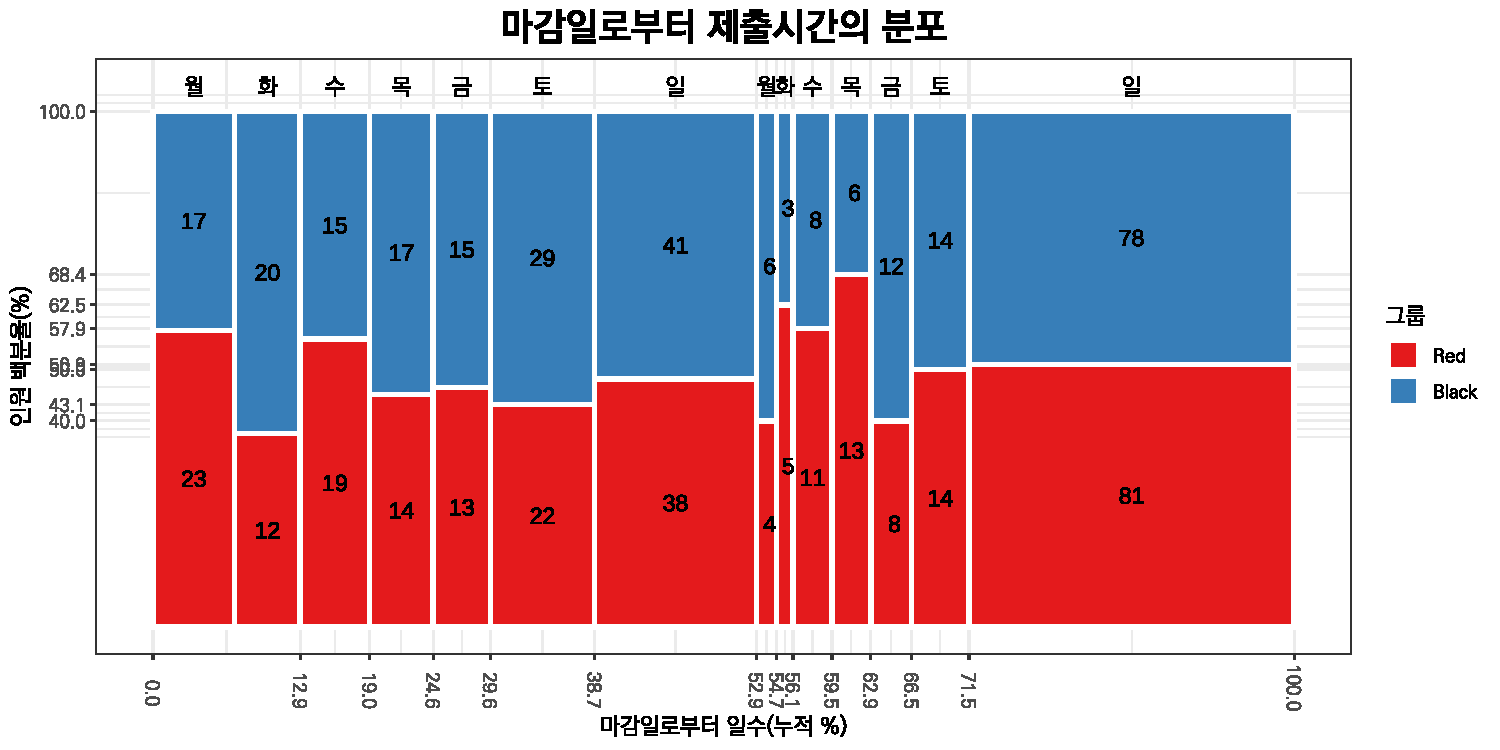
\includegraphics{quiz250331_Report_v4_files/figure-latex/unnamed-chunk-22-1.pdf}

\end{document}
